\documentclass[a4paper]{article}
\usepackage[utf8x]{inputenc}
\usepackage{natbib}
\usepackage[francais]{babel}
\usepackage{graphicx}
\usepackage[T1]{fontenc}
\usepackage[left=3cm, right=3cm, top=3cm, bottom=3cm]{geometry}
\usepackage{tikz}
\usepackage{pgfplots}
\usepackage{hyperref}
\usepackage{footnote}
\usepackage{xcolor}
\usepackage{listingsutf8}
\usepackage{verbatim}
\usepackage[bottom]{footmisc}
\usepackage{etoolbox}

\usetikzlibrary{patterns}
\pgfplotsset{compat=newest}

\setlength\parindent{0pt}
\setlength{\parskip}{1em}
\lstloadaspects{formats}



% Configure Listings
\definecolor{lightgray}{rgb}{.9,.9,.9}
\definecolor{darkgray}{rgb}{.4,.4,.4}
\definecolor{purple}{rgb}{0.65, 0.12, 0.82}

\lstdefinelanguage{JavaScript}{
	keywords={typeof, new, true, false, catch, function, return, null, catch, switch, var, if, in, while, do, else, case, break},
	keywordstyle=\color{blue}\bfseries,
	ndkeywords={class, export, boolean, throw, implements, import, this},
	ndkeywordstyle=\color{darkgray}\bfseries,
	identifierstyle=\color{black},
	sensitive=false,
	comment=[l]{//},
	morecomment=[s]{/*}{*/},
	commentstyle=\color{purple}\ttfamily,
	stringstyle=\color{red}\ttfamily,
	morestring=[b]',
	morestring=[b]"
}


\lstdefinestyle{Bash}
{language=bash,
	keywordstyle=\color{blue},
	basicstyle=\ttfamily,
	morekeywords={sudo},
	morekeywords={make},
	morekeywords={mkdir},
	morekeywords={cmake},
	morekeywords={python},
	morekeywords={pip},
	morekeywords=[2]{peter@kbpet:},
	keywordstyle=[2]{\color{red}},
	literate={\$}{{\textcolor{red}{\$}}}1 
	{:}{{\textcolor{red}{:}}}1
	{~}{{\textcolor{red}{\textasciitilde}}}1,
}


% Configure Listings
\lstset{
	inputencoding=utf8/latin1,
	basicstyle=\ttfamily,
	stringstyle=\ttfamily\color{green!50!black},
	keywordstyle=\color{blue}\bfseries,
	commentstyle=\color{red!50!black}\itshape,
	showstringspaces=true,
	breaklines=true,
	showspaces=false,
	showstringspaces=false,
	showtabs=true,  
	tabsize=2, frame=single,
	numbers=left, numberstyle=\tiny,
	firstnumber=1, stepnumber=1, numbersep=5pt,	
	moredelim=**[is][\color{red}]{@|}{@|},
	style=Bash,
	captionpos=b,
}


\newtoggle{AbstractOnly}
%\toggletrue{AbstractOnly}
\togglefalse{AbstractOnly}


\newcommand{\fyr}{\emph{Find your ride}}

% Set the docs variables
\title{Rapport \fyr}

\newcommand{\titleA}{\fyr}
\author{Lucien Camuglia}
\newcommand{\enseignants}{M. Zeltner}
\newcommand{\classe}{Classe : T.IS-E2A}
\newcommand{\ecole}{CFPT en informatique}
\newcommand{\formation}{Technicien ES en informatique}
\newcommand{\authorA}{Lucien Camuglia }
\newcommand{\travail}{Travail de diplôme}
\newcommand{\volee}{Session : 2016-2017}
\date{\today}
\newcommand{\rpi}{\emph{Raspbery Pi}}
\newcommand{\rpib}{\emph{Raspbery Pi 3 model B}}
\newcommand{\ocv}{\emph{OpenCV}}
\newcommand{\py}{\emph{Python}}
\newcommand{\gmap}{\emph{Google Maps}}
\newcommand{\bdd}{base de données}
\newcommand{\phpFolder}{../../Includes}
\newcommand{\tabitem}{~~\llap{\textbullet}~~}
% Save the values
\makeatletter

% mise en page
\usepackage{fancyhdr} 
\pagestyle{fancy} 

%En tete
\renewcommand{\headrulewidth}{1pt}
\fancyhead[L]{\@author}
\fancyhead[R]{\today}
\fancyhead[C]{\fyr}

%Pied de page
\renewcommand{\footrulewidth}{1pt}
\fancyfoot[C]{Page  \thepage}
\PassOptionsToPackage{hyphens}{url}\usepackage{hyperref}

% Spacing params
\setlength\parindent{0pt}
\setlength{\parskip}{0.75em}


\begin{document}
\begin{titlepage}
	\centering
	{\LARGE \titleA} \\
	\vspace{1cm}
	{\Large \ecole} \\
	\vspace{0.5cm}
	{\Large \formation} \\
	\vspace{0.5cm}
	{\large \travail}\\
\vspace{1cm}
\begin{figure}[ht]
\centering
\end{figure}

	\vspace{1cm}
	{\large \classe}\\
	\vspace{0.5cm}
	{\large \volee}\\
	\vspace{0.5cm}
	{\large Elève : \hfill Enseignant :}\\
    {\large \authorA  \hfill \enseignants}

	\vfill
% Bottom of the page
	{\large \today\par}
\end{titlepage}
\iftoggle{AbstractOnly}{}
{
\tableofcontents
\pagebreak}


\section{Introduction}
\subsection{Résumé}
Site WEB permettant le partage d'itinéraire entre passionné de la moto.
Ce site est réalisé en HTML/PHP/CSS/AJAX et incluant les API\footnote{\emph{Application Programming Interface}(Interface de Programation Applicative) \url{https://fr.wikipedia.org/wiki/Interface_de_programmation}} Google.

Il permet à un utilisateur de créer un trajet, de le partager et de le modifier.

Un utilisateur peut rechercher un itinéraire avec différents critères :
\begin{itemize}
    \item Durée
    \item Type de route
    \item Changement d'altitude
\end{itemize}

Le site fournit à l'utilisateur différentes données comme le temps du trajet ou la consommation théorique de la moto pour la balade.

Le motard peut aussi importer et exporter des fichiers directement depuis son GPS.


\subsection{Abstract}

The website allows sharing itineraries between motorcycle enthusiasts. The site is set-up with HTML/PHP/CSS/AJAX and Google’s API. It allows users to create trips, to share and modify them.


Different criteria can be defined by the user to create the itinerary:
\begin{itemize}
\item Travel Time
\item Type of road
\item Change in altitude, etc.
\end{itemize}



This website gives the user diverse informations. One example could be the theoretical consumption of their motorcycle for the ride or travel time. The rider can also upload or download files directly from his GPS.



\iftoggle{AbstractOnly}{
\end{document}
}{}
\pagebreak


\section{Cahier des charges}
TODO inclure le CDC


\pagebreak

\section{Analyse de l'existant}


\subsection{Garmin BaseCamp}
Garmin BaseCamp est un logiciel fournit par Garmin.

Il permet à un utilisateur de créer un trajet et de l'importer sur son GPS.

Il donne aussi la possibilités a l'utilisateur de visionnée ses différent déplacement.

\begin{tabular}{|l|l|}
\hline
   Positif & Négatif \\
   \hline
   \hline
   \tabitem Connexion directe avec le GPS & \tabitem Pas de partage\\
   &\tabitem Obligation de posseder un GPS Garmin\\
   \hline
 \end{tabular}
 
\subsection{http://www.calculitineraires.fr/}

www.calculitineraires.fr est un site de partage d'itinéraire pour la course à pied, le vélo et la randonnée

Il permet l'import/export de fichier GPX et TCX, la rechercher et le partage d'itinéraire.

\begin{tabular}{|l|l|}
\hline
   Positif & Négatif \\
   \hline
   \hline
   \tabitem Assez complet & \tabitem Interface compliquée d'utilisation\\
   \tabitem Import / Export des fichiers GPS &\tabitem Pas de contribution pour la moto\\
   \tabitem Création d'itinéraire & \\
   \hline
 \end{tabular}


\subsection{http://www.bestbikingroads.com}
www.bestbikingroads.com est un site de partage d'itinéraire moto.


Il permet l'import/export de fichier GPX, la rechercher, le partage d'itinéraire ainsi que la notation des balades.

\begin{tabular}{|l|l|}
\hline
   Positif & Négatif \\
   \hline
   \hline
   \tabitem Assez complet & \tabitem Tout les tracés s'affiche en meme temps sur la carte\\
   \tabitem Import / Export des fichiers GPS & \tabitem pas de modification possible\\
   \tabitem Création d'itinéraire & \\
   \tabitem Notation des balades & \\
   \hline
 \end{tabular}



\pagebreak

\section{Analyse fonctionnelle}

\subsection{Généralités}
Ci-dessous se trouve le schéma initial de mon site web. Les ronds représentent des pages et les flèches entre ceux-ci représentent d'éventuelles actions ou états.

\begin{figure}[h]
\centering
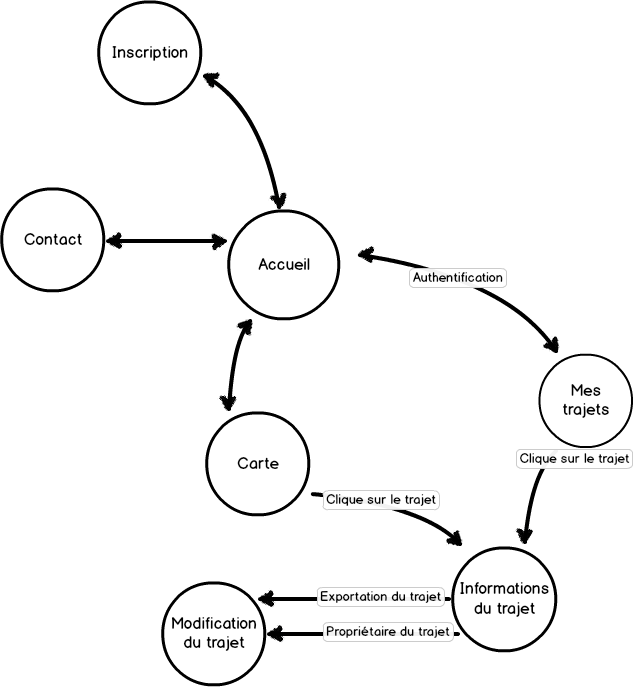
\includegraphics[width=\textwidth]{./Images/ShemaSite.png}
\caption{Schéma du site}
\end{figure}

\subsection{Description des fonctionnalités globales}
\subsubsection{Connexion}
Cette fonctionnalité permet à un utilisateur de s'authentifier et d'accéder à ses trajets mit en ligne ou partager de nouveaux trajets.

\subsubsection{Inscription}
Cette fonctionnalité permet à un nouvel utilisateur de créer un compte et donc de pouvoir bénéficier des fonctionnalités d'un utilisateur connecté

\subsubsection{Création de trajet}
Cette fonctionnalité se distingue en deux sous fonctionnalités : 
\begin{itemize}
    \item Création : crée un nouveau trajet depuis le site directement.
    \item Importation : importe un fichier de type GPX et éventuellement modifier le trajet.
\end{itemize}

\subsubsection{Exportation}
Cette fonctionnalité permet à un utilisateur d'exporter le trajet de son choix au format GPX pour l'inclure dans son GPS.

\subsubsection{Suppression d'un trajet}
Cette fonction permet a un utilisateur de supprimer un de ses trajet.

\subsubsection{Visualiser le trajet}
Cette fonctionnalité permet à n'importe qui de visualiser les trajets mit en ligne, puis les exporter en les modifiant s'il le souhaite.

\newpage

\subsection{Description de l'interface}

\subsubsection{Inscription}
\begin{figure}[h]
\centering
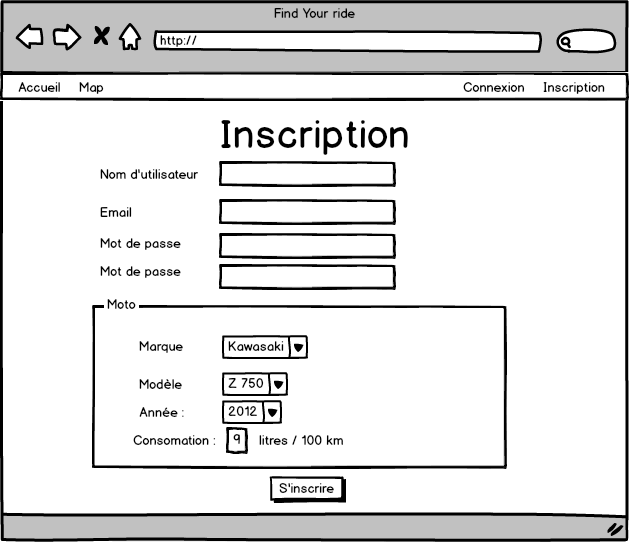
\includegraphics[width=0.5\textwidth]{./Images/Interfaces/inscription.png}
\caption{Page inscription}
\end{figure}

Cette page sert à l'inscription des utilisateurs. On y trouve différent champs : 
\begin{itemize}
    \item Nom d'utilisateur
    \item E-mail
    \item Mot de passe, ce champ apparaît deux fois pour avoir la validation de celui-ci
    \item Moto : diverse informations sur la moto de l'utilisateur comme par exemple sa con somation pour calculer la con somation des trajets. Le champ \emph{Moto} est facultatif mais conseillé.
\end{itemize}

\subsubsection{Map}
\begin{figure}[h]
\centering
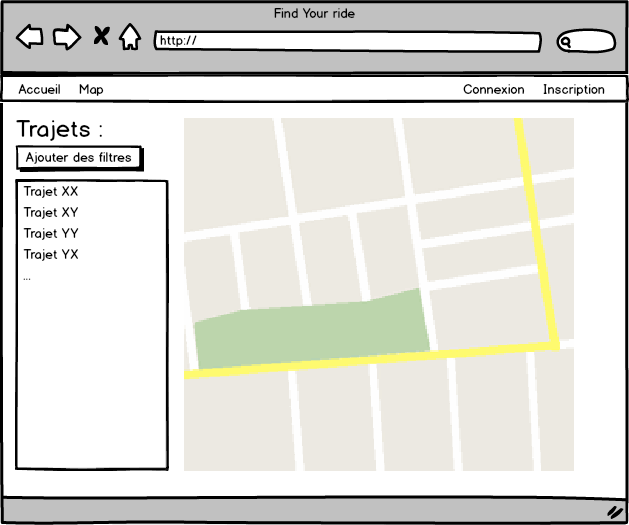
\includegraphics[width=0.5\textwidth]{./Images/Interfaces/Map.png}
\caption{Page inscription}
\end{figure}

Cette page sert à l'affichage de la carte et des différents trajets.

Sur la gauche apparaissent tout les trajets ainsi qu'un bouton filtre.
Ce bouton permet de filtre les trajets parmi différents critères.
\begin{itemize}
    \item Avec ou sans autoroute
    \item Durée
    \item Dénivelé
    %\item sinuosité
\end{itemize}
Sur la droite une carte Google ou apparaît le tracé sélectionné.

\subsubsection{Detail trajet}
\begin{figure}[h]
\centering
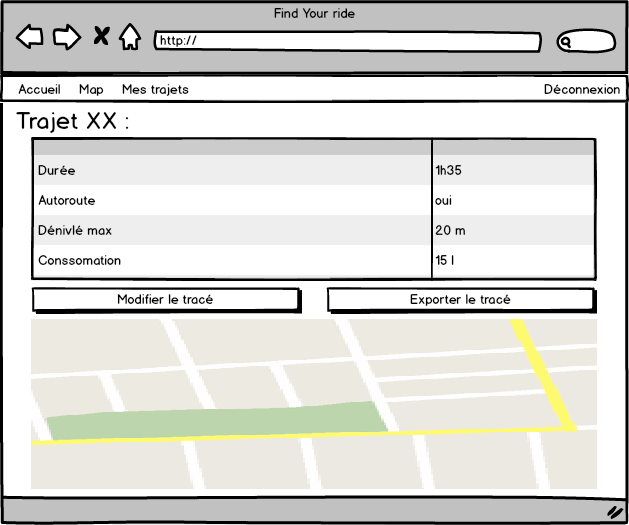
\includegraphics[width=0.5\textwidth]{./Images/Interfaces/DetailTrajet.png}
\caption{Page Detail Trajet}
\end{figure}

Cette page sert à afficher le détail d'un trajet.

Sur le haut de la page apparai les détails du trajet.
\begin{itemize}
    \item Durée du trajet
    \item S'il contient des autoroutes
    \item Dénivelé
    \item La consomation (si l'utilisateur à renseignée les données de la moto)
    %\item sinuosité
\end{itemize}
Deux bouton sont présent pour modifier ou exporter le trajet.
Sur le bas de la page, la carte google avec le trajet.

\subsubsection{Connexion}
\begin{figure}[h]
\centering
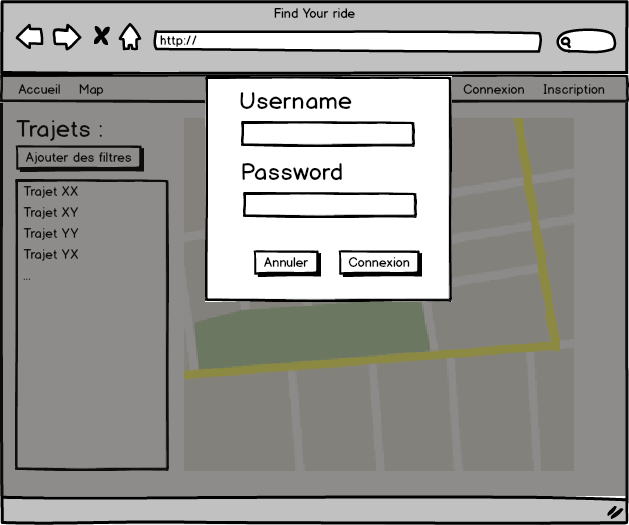
\includegraphics[width=0.5\textwidth]{./Images/Interfaces/Connexin.png}
\caption{Modal connexion}
\end{figure}

Le formulaire de connexion est une fenêtre modal qui s'ouvre par dessus les autres pages avec uniquement deux champs.
\begin{itemize}
    \item Nom d'utilisateur
    \item Mot de passe
\end{itemize}


\subsubsection{Vos trajets}
\begin{figure}[h]
\centering
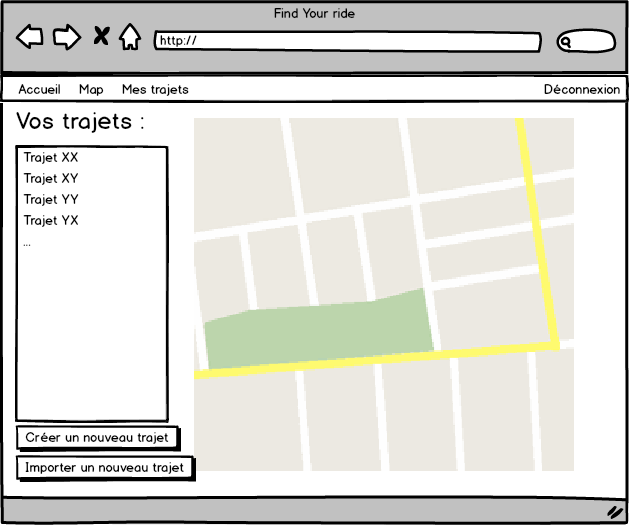
\includegraphics[width=0.5\textwidth]{./Images/Interfaces/VosTrajets.png}
\caption{Page vos trajet}
\end{figure}

Cette page est identique que la page \emph{Map} mais au lieu d'avoir tout les trajet disponible du site, il y a uniquement les trajet de l'utilisateur.

Deux boutons sont disponible sur cette page.
\begin{itemize}
    \item Créer un nouveau trajet, permet de créer un trajet a partir de la carte
    \item Importer un nouveau trajet, permet d'importer un fichier GPX avec le trajet.
\end{itemize}

\subsection{Description des éléments de sécurité}
\subsubsection{Fichier .htaccess}
Permet d'empêcher la navigation sur certain dossier/fichiers du site. Ils permettent aussi de définir des pages d'erreurs personnalisées

\subsubsection{Utilisateur de la base de données}
Utiliser un utilisateur différent que \emph{root} pour accéder à la base de donnée afin de donner des droits qu'au éléments nécessaire.

\subsubsection{Requêtes}
Utilisation de requêtes préparée pour éviter les injections SQL.


\pagebreak








\pagebreak


\section{Analyse organique} 
\subsection{Résumé}
Dans cette section sera expliquer le fonctionnement de l'application.


\subsection{Google API}
Les API\footnote{\emph{Application Programming Interface}(Interface de Programation Applicative) \url{https://fr.wikipedia.org/wiki/Interface_de_programmation}} Google sont une suite d'outils développé et fourni par Google pour permettre à des utilisateurs d'intégrer les services Google dans un site web ou une application.

Il en existe environ 66 dont 16 pour \gmap. Pour la réalisation de ce site j'utilise 4 API \gmap : 
\begin{itemize}
    \item Google Maps Javascript
    \item Google Direction
    \item Google Elevation
    \item Google Roads
\end{itemize}

\subsubsection{Google Maps Javascipt}
Cette API permet d'intégrer une \gmap sur le site web, c'est la seule qui sera visible pour l'utilisateur. C'est sur celle-ci qu'apparaissent les itinéraires et les positions GPS.
\subsubsection{Google Direction}
Le fonctionnement de cette API est assez simple. Il suffit d'envoyer un point d'origine et une destination à Google Direction et il nous retourne un tableau JSON avec différent paramètres.
\begin{itemize}
    \item La durée
    \item La distance
    \item Les étapes du parcours (positions GPS)
    \item Les étapes du parcours (Francais, par exemple : Tournez a droite,...)
\end{itemize}

\subsubsection{Google Elevation}
TODO
\subsubsection{Google Roads}
Cette API permet de faire 3 choses différentes :
\begin{itemize}
    \item \emph{Snap to raod}
    \item \emph{Nearest road}
    \item \emph{Speed limits}
\end{itemize}

J'utilise deux fonctionnalitées de cette API, \emph{Snap to raod} et \emph{Nearest road}.

\emph{Snap to raod} permet de "déplacer" un trajet pour qu'il suive la route. Il faut lui envoyer l'ensemble des point GPS de notre route et il nous retourne un ensemble de point qui suivent la route.

\emph{Nearest road} permet de donner la position d'un point GPS sur la route la plus proche.

\subsection{Fonction PHP pour la \bdd}
\subsubsection{connexion à la \bdd}
La connexion à la \bdd se fait à l'aide de PDO\footnote{\emph{PHP Data Object}, \url{http://php.net/manual/fr/intro.pdo.php}}. PDO a besoin de l'utilisateur de la \bdd et du mot de passe ainsi que le nom de la base.
Je lui précise aussi le mode d'erreur qui est \emph{PDO::ERRMODE\_EXCEPTION} ce mode permet d'afficher le code d'erreur et de déclencher une exception\footnote{Plus d'informations \url{http://php.net/manual/fr/pdo.error-handling.php}}.

Afin d'avoir un partage d'informations dans le bon format, on défini l'encodage de caractères en UTF-8

\lstinputlisting[language=php,firstline=14,lastline=35]{../../Includes/functions.php}
\subsubsection{Requête préparée}
Afin de sécuriser le site et éviter les injections SQL j'utilise des requête préparée.

On commence par préparer la requête, PDO va substituer les marqueurs (\emph{:marqueur}) pour les valeur fournie dans le tableau de paramètres fourni au moment de l'exécution. Ensuite, il faut exécuter la requête avec les parametres.
\lstinputlisting[language=php,firstline=45,lastline=52]{../../Includes/functions.php}


\newpage
\subsection{Inscription sur le site}

Afin de pouvoir bénéficier de toutes les fonctionna litées du site, l'utilisateur doit se connecter. Si celui-ci n'a pas de compte, il a la possibilité d'un créer un. 

La création d'un utilisateur se fait en plusieurs étapes :
\begin{itemize}
    \item Contrôle en AJAX lors de la saisie des informations par l'utilisateur
    \item Contrôle en PHP des informations
    \item Création de l'utilisateur en PHP et SQL
\end{itemize}

La vérification Ajax est assez simple, lorsque l'utilisateur appuye sur une touche, on affiche une croix rouge puis on envoie une requete à la page PHP qu va nous retourner un booléen a \emph{true} si l'utilisateur exite. S'il est vrai, on laisse la croix rouge sinon on affiche un vu vers.
\lstinputlisting[firstline=124,lastline=141]{../../JS/Signin.js}
\lstinputlisting[firstline=62,lastline=79]{../../JS/Signin.js}
Une fois la verification faite en javascript/ajax, les données sont envoyées a une fonction PHP qui revérifie si l'utilisateur est déjà présent dans la base, puis, récupère l'identifiant de la moto daprès la marque, le model et l'année.
Finalement, les données sont ajoutée à la base de données.
\lstinputlisting[language=php,firstline=166,lastline=198]{../../Includes/functions.php}


\subsection{Connexion au site}
Une fois l'inscirption effectuée, l'utilisateur a la possibilité de se connecter au site.

Pour ce faire, l'utilisateur saisi ses informations dans le formulaire et se connecte.
Une première vérification en HTML5 vérifie que les champs soient remplis(\emph{required}).
Une fois cette vérification éffectuée, les informations sont envoyée à la page PHP \emph{connexion.php} qui vérifie encore une fois que les champs soient rempli. Puis, envoie les données à la fonction PHP de connexion qui va récupérer :
\begin{itemize}
	\item Les ids utilisateur
	\item Les mots de passe
	\item Les roles
\end{itemize}

Une fois ces informations récupérée, on tous les parcourir pour être sûr que le nom d'utilisateur et le mot de passe fourni correspondent bien à un utilisateur existant.
Si c'est le cas, on enregistre l'id, le role et le nom d'utilisateur dans des \emph{Sessions} et on retourne \emph{true} pour dire que les informations sont correcte.


\lstinputlisting[language=php,firstline=8,lastline=33]{../../Includes/connexion.php}
\lstinputlisting[language=php,firstline=60,lastline=86]{../../Includes/functions.php}

\begin{comment}


\end{comment}

\pagebreak

\section{Problèmes rencontré}
\subsection{Google Api}
\subsection{Async}

\begin{comment}


Je ne connaissai pas le python ce qui fait qu'il m'a fallut un peu de temps avant de comprendre la syntaxe et l'utilisation.
Deplus, je n'aavais jamais utiliser de module GSM, je ne connaissai pas les commandes AT ni le fonctionnement de celles-ci.

Un gros problème que j'ai rencontré est que le \rpi n'est pas assez puissant pour alimenter le modem GSM. Comme je ne le savais pas, j'ai mit plusieurs semaines avant de m'en rendre compte. La solution serai d'uiliser un HUB USB utilisant une allimentation externe.

\pagebreak
\end{comment}
\section{Conclusion}
\begin{comment}


Ce projet a été très intéressent de part la decouvert du \emph{Python} et l'utilisation des commandes AT.
Il est compliqué dans un délai aussi court d'apprendre de nouvelles technologies et de les appliquer. Mon projet est fonctionnel (ormis l'envoie de SMS) et je suis plutot contant du résultat. Je finirais completement ce projet chez moi afin de pouvoir le déplyoyer comme il était prévu à l'origine.
\end{comment}
\pagebreak



\listoffigures

\end{document}